\section{Systembeschreibung}{161}

Ein System transformiert mindestens ein Eingangssignal $x(t)$ in mindestens ein Ausgangssignal $y(t)$.
Die Zuordnung zwischen Eingang und Ausgang muss \textbf{eindeutig} sein! \\
Die Transformation erfolgt mittels Übertragungsfunktion $H(s)$ (UTF)

\vspace{-0.6cm}

\begin{center}
    $$ \boxed{H(s) = \frac{Y(s)}{X(s)}} $$
    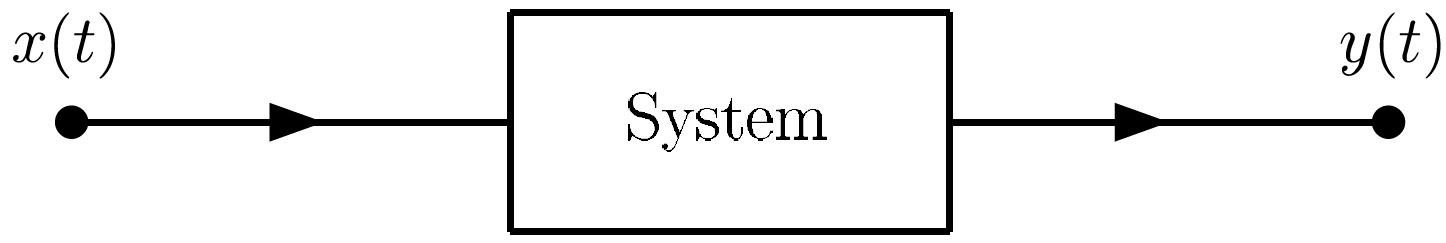
\includegraphics[width=0.75\columnwidth]{images/system.png}
\end{center}


\subsection{Eingangs-zu-Ausgangsbeziehungen }{161}

\begin{tabular}{ll}
    SISO & Single Input Single Output       \\
    MIMO & Multiple Input Multiple Output   \\
    MISO & Multiple Input Single Output 
\end{tabular}


\subsubsection{Wirkungsfreiheit}{161-162}

\begin{itemize}
    \item Systemausgänge dürfen nachfolgende Systeme nicht beeinflussen
    \item Systemeingänge dürfen vorhergehende Systeme nicht beeinflussen
\end{itemize}

\vspace{-0.2cm}

\begin{center}
    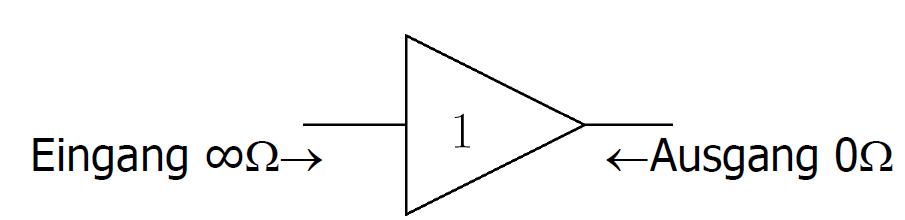
\includegraphics[width=0.7\columnwidth]{images/wirkungsfreiheit.png}
\end{center}


\subsection{Invertierbare vs. nichtinvertierbare System}{173}

\subsubsection{Invertierbare Systeme}

Ein System wird als \textbf{invertierbar} bezeichnet, wenn bei jedem Ausgangssignal \textbf{eindeutig} auf das entsprechende 
Eingangssignal geschlossen werden kann.

\vspace{0.2cm}

\example{(Nicht) Invertierbare Systeme}

\begin{minipage}[t]{0.48\columnwidth}
    $y = x^2$ \quad \textrightarrow\ nicht invertierbar
\end{minipage}
\hfill
\begin{minipage}[t]{0.48\columnwidth}
    $y = x^3$ \quad \textrightarrow\ invertierbar 
\end{minipage}


\subsection{Reelle Systeme vs. komplexwertige Systeme}{173}

Ein System wird als \textbf{reell} bezeichnet, wenn ein \textbf{relles Eingangssignal} immer ein \textbf{reelles Ausgangssignal} bewirkt.


\subsection{Statische vs. Dynamische Systeme}{162-163}

\subsubsection{Statische (resistive) Systeme (System ohne Gedächtnis)}


Der Wert des Ausgangssignals $y(t_0)$ zum gegenwärtigen Zeitpunkt $t_0$ \textbf{hängt nur vom gegenwärtigen Wert des Eingangs $\bm{x(t_0)}$ ab}. \\
Systembeschreibung: algebraische Gleichungen 
$$ \boxed{ y(t_0) = f\{x(t_0) \} \, \forall \, t_0  } $$


\subsubsection{Dynamische Systeme (System mit Gedächtnis)}

Der Wert des Ausgangssignals $y(t_0)$ zum gegenwärtigen Zeitpunkt $t_0$ \textbf{hängt auch von anderen Zeitpunkten als $\bm{t = t_0}$ ab}. \\
In elektrischen Systemen wirken $L$ und $C$ als Speicherelemente und machen ein System dynamisch. \\
Systembeschreibung: Differentialgleichungen


\subsection{Kausale vs. akausale Systeme}{164}

\begin{itemize}
    \item \textbf{Alle statischen} Systeme sind \textbf{kausal} 
    \item \textbf{Nicht alle kausalen} Systeme sind \textbf{statisch}
\end{itemize}



\subsubsection{Kausale Systeme}

Der Wert des Ausgangssignals $y(t_0)$ hängt nur von Eingangssignalen $x(t \leq t_0)$ ab. \\
\textrightarrow\ 'Das System kann \textbf{nicht} in die Zukunft schauen' \\
\vspace{0.1cm}
\crd{\textbf{Physikalische Systeme sind immer kausale Systeme!}}


\subsubsection{Akausale Systeme}

Der Wert des Ausgangssignals $y(t_0)$ hängt auch von \textbf{zukünftigen} Eingangsignalen $x(t > t_0)$ ab. \\
\textrightarrow\ 'Das System sieht in die Zukunft' 


\subsection{Lineare vs. nichtlineare Systeme}{165-166}

\subsubsection{Lineare Systeme}

Bei einem linearen System gilt das \textbf{Superpositionsprinzip} 
$$ \boxed{   \{a \cdot x_1(t) + b \cdot x_2(t) \} = a \cdot f \{ x_1(t)   \} + b \cdot f \{ x_2(t) \} } $$

\textbf{\textrightarrow\ Alle Systeme, die nur als $\bm{R}$, $\bm{L}$ und $\bm{C}$ bestehen, sind linear.} 

\vspace{0.2cm}

Alle Differentialgleichungen der Form
$$ \boxed{ \sum\limits_{i=0}^n  a_i \frac{\diff^i y(t) }{\diff t^i} = \sum\limits_{j=0}^m  b_j \frac{\diff^j x(t) }{\diff t^j} \, \laplace \, Y(s) \cdot \sum\limits_{i=0}^n a_i s^i = X(s) \cdot \sum\limits_{j=0}^m b_j s^j } $$
beschreiben ein lineares, kausales, zeitinvariantes System (LTI-System).


\subsubsection{Nichtlineare Systeme}{167}

Ein System, welches bei \textbf{kurzgeschlossenem Eingang} ($x(t) = 0$) ein \textbf{Ausgangssignal} hat ($y(t) \neq 0$), 
ist ein \textbf{nichtlineares} System.

\vspace{0.1cm}

\textrightarrow\  Nichtlineare Systeme erlauben das Erzeugen \textbf{neuer Frequenzanteile}.

\vspace{0.2cm}
\myul{\textbf{Beispiel:}}

\vspace{0.1cm}
Gerade, welche nicht durch Ursprung geht


\subsection{Zeitinvariante vs. zeitvariante Systeme}{170}

\subsubsection{Zeitinvariante Systeme}

Ein System ist \textbf{in}variant, wenn eine zeitliche Verschiebung des Eingangssignals $x(t)$ um eine feste Zeit $t_0$ 
eine \textbf{gleich grosse Zeitverschiebung am Ausgang} bewirkt aber die Form des Signals nicht ändert.

$$ \boxed{ x(t) \to y(t), \text{ dann gilt } x(t- t_0) \to y(t- t_0) \, \forall \, t_0  } $$

Trifft dies nicht zu, so handelt es sich um ein \textbf{zeitvariantes} System.


\subsubsection{Zusammenhänge bei statischen Systemen}{170}

\begin{center}
    \begin{tabular}{lll}
        \toprule
        \textbf{Zusammenhang}                   & \textbf{Mathemetische Darstellung}        & \textbf{Beispiel}         \\
        \midrule
        linear \& zeit\textbf{in}variant        & $y(t) = \gamma \cdot x(t)$                & $y(t) = 3 \cdot x(t)$     \\
        \midrule
        linear \& zeitvariant                   & $y(t) = \gamma(t) \cdot x(t)$             & $y(t) = t^2 \cdot x(t)$   \\
        \midrule
        nichtlinear \& zeit\textbf{in}variant   & $y(t) = f\{x(t)\}$                        & $y(t) = 4 \cdot x^2(t)$   \\
        \midrule
        nichtlinear \& zeitvariant              & $y(t) = f\{x(t), \, t\}$                  & $y(t) = t \cdot x^3(t)$   \\
        \bottomrule
    \end{tabular}
\end{center}

